\documentclass[../sparc.tex]{subfiles}
\graphicspath{{\subfix{../images/}}}
\begin{document}

%%%%%%%%%%%%%%%%%%%%%%%%%%%%%%%%%%%%%%%%%%%%%%%%%%%%%%%%%%%%%%%%%%%%%%%%%%%%%%%%
\section{Реализация игровой карты}
\index{Двумерные массивы}

В играх вокруг игрока обычно разворачивается некоторое действие -- не-игровые
персонажи (Non-Playable Characters, сокращённо ``NPC'') ревностно патрулируют
территорию карты; появляются и исчезают различные объекты, с которыми можно
взаимодействовать; наконец, повсюду располагаются различные \emph{статические}
объекты, которые могут преграждать путь игроку, или же являться просто
элементами декора.

Простым способом расположить отдельный объект на карте является задание ему
координат на карте и отрисовка -- так же, как мы делаем это с игровым
персонажем.  Однако при создании двух переменных (для координаты по оси X и по
оси Y) на каждый объект, количество переменных будет расти очень быстро.  Только
представьте, что карта размером 20х4 может потенциально хранить 80 объектов, что
даёт суммарно 160 переменных для адресации каждого из них!  Для решения этой
проблемы мы должны прибегнуть к уже известным нам массивам, с одной оговоркой --
мы должны будем использовать \emph{двумерные массивы}.

Схематическое изображение двумерного массива можно увидеть на
рис. \ref{fig:2d-array-example}.

\begin{figure}[ht]
  \centering
  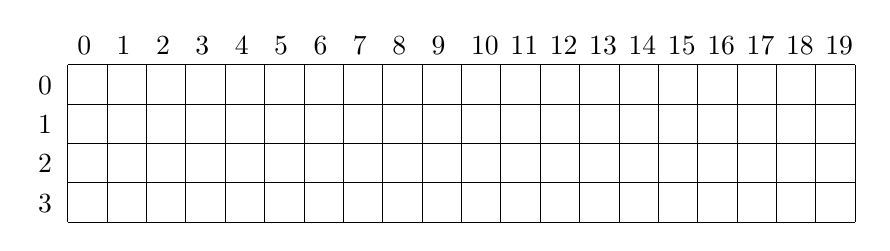
\begin{tikzpicture}
    \draw[step=0.5cm,black,very thin] (-5, -2) grid (5, 0);
    \foreach[count=\n from 0] \x in {-5, -4.5, ..., 4.5} {
      \draw (\x cm, 0) node[anchor=south west] {$\n$};
    }
    \foreach[count=\n from 0] \y in {-0.5, -1.0, ..., -2} {
      \draw (-5.5, \y) node[anchor=south west] {$\n$};
    }
  \end{tikzpicture}
  \caption{Схематическое изображение массива 4x20 (4 строки, 20 столбцов.)}
  \label{fig:2d-array-example}
\end{figure}

Можно также представить двумерный массив 4x20, как одномерный массив из 4-х
элементов, каждая ячейка которого содержит ссылку на ещё один одномерный массив
длиной 20 ячеек, как показано на
рис. \ref{fig:2d-array-example-with-references}.

\begin{figure}[ht]
  \centering
  \begin{tikzpicture}
    \draw[step=0.5cm,black,very thin] (-5, -2) grid (-4.5, 0);
    \draw[step=0.5cm,black,very thin] (-4, -2) grid (6, 0);
    \foreach[count=\n from 0] \x in {-4, -3.5, ..., 5.5} {
      \draw (\x cm, 0) node[anchor=south west] {$\n$};
    }
    \foreach[count=\n from 0] \y in {-0.5, -1.0, ..., -2} {
      \draw (-5.5, \y) node[anchor=south west] {$\n$};
    }
    \foreach[count=\n from 0] \y in {-0.25, -0.75, ..., -2} {
      \draw[{Circle}-{Stealth}]  (-4.8, \y) -- (-4, \y);
    }
  \end{tikzpicture}
  \caption{Схематическое представление массива 4x20 в виде одномерного массива
    из 4-х элементов со ссылками на одномерные массивы по 20 элементов.}
  \label{fig:2d-array-example-with-references}
\end{figure}

Для наших задач реализации игры нам потребуется задать массив, хранящий тип
данных \texttt{char}.  Размер нашего массива -- нашей игровой карты -- мы
зададим с помощью именованных констант, где-нибудь в глобальной области кода,
выше \texttt{setup}.

\begin{minted}{cpp}
  const int MAP_W = 20; // Ширина карты.
  const int MAP_H = 4;  // Высота карты.
\end{minted}

Далее создадим сам двумерный массив, который станет нашей игровой картой.

\begin{minted}{cpp}
  char game_map[MAP_H][MAP_W];
\end{minted}

Обратите внимание, что при объявлении массива используется две пары квадратных
скобок.  В первой паре скобок задаётся высота массива (количество строк), во
второй -- ширина массива (количество столбцов.)

Далее нам необходимо объявить функцию отображения карты на экране -- назовём её
\texttt{map\_show}.

\begin{minted}{cpp}
  void map_show() {
    for (int y = 0; y < MAP_H; y++) {
      for (int x = 0; x < MAP_W; x++) {
        lcd.setCursor(x, y);
        lcd.print( game_map[y][x] );
      }
    }
  }
\end{minted}

Как мы видим, тело функции состоит из двух вложенных друг в друга циклов
\texttt{for}.  Первый из циклов, идущий по \texttt{y}, перебирает строки
массива.  Второй цикл по \texttt{x} перебирает столбцы.  Поскольку цикл по
\texttt{x} вложен в цикл по \texttt{y}, то на каждое изменение \texttt{y}
происходит полный проход цикла по \texttt{x}.

Во вложенном цикле у дисплея вызывается функция \texttt{setCursor} для указания
позиции вывода символа на экран.  Далее символ печатается в указанную клетку
через \texttt{print}.

Поскольку массив \texttt{game\_map} имеет тип \texttt{char}, то символы,
хранящиеся в нём, автоматически выводятся на дисплей в правильном виде -- а
именно, как графические символы, а не их коды в таблице символов.

Функцию \texttt{map\_show} необходимо вызвать в \texttt{loop} для того, чтобы
карта отобразилась на экране.

\begin{minted}{cpp}
  void loop() {
    if (digitalRead(BUTTON_R) == LOW) {
      // ...
    }
    if (digitalRead(BUTTON_L) == LOW) {
      // ...
    }

    // Вызов функции отрисовки карты на экране дисплея.
    map_show();

    // Отрисовка игрока поверх карты.
    lcd.setCursor(player_x, player_y);
    lcd.print(PLAYER);

    // Задержка, чтобы избежать слишком быстрого считывания
    // нажатий на кнопки.
    delay(100);
  }
\end{minted}

Обратите внимание, что отрисовка карты выполняется перед отрисовкой игрока.
Если поменять этот порядок, то тогда игрок не будет виден на экране, ведь его
изображение будет перетёрто отрисовкой карты.

После загрузки и запуска данной программы вы можете обнаружить, что дисплей
наполнился случайными символами.  Это произошло потому, что мы не
инициализировали массив \texttt{game\_map} значениями, и там сейчас во всех
ячейках \emph{мусор} -- то есть, какие-то неожиданные значения.

Чтобы исправить эту ситуацию, нам необходимо создать функцию генерации карты,
которая будет заполнять карту чем-то вменяемым.  Для начала заполним карту
пробелами, которые будут у нас символизировать пустое место на карте.

В глобальной области перед \texttt{setup} зададим специальную константу для
обозначения пустого места.

\begin{minted}{cpp}
  const char SPACE = ' ';    // Пустое пространство.
\end{minted}

Теперь мы можем использовать константу \texttt{SPACE} для задания пустого места.

Перейдём к описанию функции генерации карты.

\begin{minted}{cpp}
  void map_generate() {
    for (int y = 0; y < MAP_H; y++) {
      for (int x = 0; x < MAP_W; x++) {
        game_map[y][x] = SPACE;
      }
    }
  }
\end{minted}

Как можно видеть, функция \texttt{map\_generate} не сильно отличается от функции
\texttt{map\_show}.

Функцию \texttt{map\_generate} необходимо вызвать один раз внутри функции
\texttt{setup}.

\begin{minted}{cpp}
  void setup() {
    lcd.init();
    lcd.backlight();

    // Настройка кнопок управления.
    pinMode(BUTTON_R, INPUT_PULLUP);
    pinMode(BUTTON_L, INPUT_PULLUP);

    // Вызов функции генерации карты.
    map_generate();
  }
\end{minted}

После загрузки новой прошивки в Arduino, мы должны увидеть экран, где
отображается только игрок, поскольку карта у нас ``пустая'' (заполнена
пробелами.)

Теперь мы получили возможность размещать на карте объекты.  Начнём с добавления
нового игрового объекта -- пусть это будет ``стена'', т.е. непроходимый участок
карты.  Зададим стену в виде символа ``\#''.

\begin{minted}{cpp}
  const char SPACE = ' ';    // Пустое пространство.
  const char WALL  = '#';    // Стена.
\end{minted}

После этого мы можем разместить этот объект на карте, модифицировав функцию
\texttt{map\_generate}.  Добавим несколько стен.

\begin{minted}{cpp}
  void map_generate() {
    for (int y = 0; y < MAP_H; y++) {
      for (int x = 0; x < MAP_W; x++) {
        game_map[y][x] = SPACE;
      }
    }

    // Добавляем вручную на карту объекты.
    game_map[0][10] = WALL;
    game_map[1][10] = WALL;
    game_map[2][10] = WALL;
  }
\end{minted}

После загрузки программы в Arduino, мы увидим, что объекты появились на экране.
Таким образом мы можем разместить и другие объекты.  Однако возникает другая
проблема -- как игроку взаимодействовать с ними?  В текущей реализации игрок
свободно проходит сквозь стены, как привидение.  Решение этой проблемы как раз
описано в следующем разделе.

%%%%%%%%%%%%%%%%%%%%%%%%%%%%%%%%%%%%%%%%%%%%%%%%%%%%%%%%%%%%%%%%%%%%%%%%%%%%%%%%
\subsubsection{Задачи}
\begin{enumerate}
\item Объявите дополнительные игровые объекты в виде символьных констант, как мы
  это делали со \texttt{SPACE} и \texttt{WALL} -- например, можно добавить
  ``дверь'' на следующий уровень, или же особый вид стен.
\item Добавьте дополнительные объекты на карту, для создания желаемого игрового
  мира.
\end{enumerate}

%%%%%%%%%%%%%%%%%%%%%%%%%%%%%%%%%%%%%%%%%%%%%%%%%%%%%%%%%%%%%%%%%%%%%%%%%%%%%%%%
\subsection{Взаимодействие игрока с объектами}

Возможно, вам доводилось работать в графических редакторах вроде GNU Image
Manipulation Program (GIMP) -- подобные ``продвинутые'' редакторы позволяют
создавать многослойные изображения.  На отдельно взятом слое могут быть
прозрачные области, сквозь которые виден нижележащий слой.  Таким образом можно
создавать сложные композиции.  Тем не менее, при экспорте изображения в
растровый графический формат (например, PNG) все эти слои объединяются в один
слой, снизу вверх -- то есть, каждый следующий слой накладывается на предыдущий
с учётом прозрачности.

Мы можем представить себе игровой мир, как подобный набор ``слоёв''.  На данный
момент у нас два слоя -- самый нижний (назовём его нулевым) хранит объекты
нашего мира (это как раз массив \texttt{game\_map}).  Слой выше (назовём его
первым) хранит игрока.

Для того, чтобы игрок на первом слое мог взаимодействоать с игровыми объектами
на нулевом, нам необходимо сделать сопоставление позиции игрока с содержимым
нулевого слоя.

Для примера попробуем сделать так, чтобы игрок не мог проходить сквозь стены.
Если игрок пытается идти вправо на клетку, и там -- стена, тогда мы не меняем
позицию игрока. Если же справа от игрока находится пустая клетка, то меняем
позицию.  Пример того, как это можно реализовать в коде, показан ниже.

\begin{minted}{cpp}
  void loop() {
    if (digitalRead(BUTTON_R) == LOW) {
      if (player_x < 15) {
        // Проверяем, что находится справа от игрока.
        if (game_map[player_y][player_x + 1] != WALL) {
          // Если справа не стена, то тогда позволяем
          // игроку сместиться на одну клетку вправа.
          player_x++;
        }
      }
    }

    // ...
  }
\end{minted}

Здесь следует обратить особое внимание на данный код.

\begin{minted}{cpp}
  if (game_map[player_y][player_x + 1] != WALL) {
    // ...
  }
\end{minted}

Как мы помним, \texttt{game\_map} хранит игровую карту.  Для того, чтобы узнать,
что находится на клетке карты справа от игрока, мы подставляем в качестве номера
строки массива значение \texttt{player\_y}, а в качестве номера столбца
подставляем \texttt{player\_x + 1} (прибавление единицы как раз позволяет от нас
взять следующую клетку.)  Затем полученное из массива значение сравнивается с
константой \texttt{WALL} -- мы проверяем, что значение не равно (``!='') данной
константе.

Поскольку мы будем подобные сравнения использовать достаточно часто, имеет смысл
сделать специальные функции для проверки клеток карты на наличие определённых
объектов.  Например, мы можем создать вспомогательную функцию подобного рода:

\begin{minted}{cpp}
  // Функция, возвращающая 1 (true) в случае, если
  // на клетке карты по координатам x,y находится стена.
  // В противном случае функция возвращает 0 (false).
  bool is_wall(int x, int y) {
    return game_map[y][x] == WALL;
  }
\end{minted}

\note{
  В языке C++ значение 0 означает ``ложь'' (``false''), тогда как любое ненулевое
  значение означает истину (например, числа 1, 42, -41 и т.п. являются значением
  ``истина'' с точки зрения языка.)
}

Используя новую функцию \texttt{is\_wall} код внутри \texttt{loop} можно будет
свести к следующему виду:

\begin{minted}{cpp}
  void loop() {
    if (digitalRead(BUTTON_R) == LOW) {
      if (player_x < 15) {
        // Проверяем, что находится справа от игрока.
        if (! is_wall(player_x + 1, player_y)) {
          // Если справа не стена, то тогда позволяем
          // игроку сместиться на одну клетку вправа.
          player_x++;
        }
      }
    }

    // ...
  }
\end{minted}

Обратите внимание на эту часть кода:

\begin{minted}{cpp}
  if (! is_wall(player_x + 1, player_y)) {
    // ...
  }
\end{minted}

Используется знак ``!'', который означает логическое отрицание (``НЕ''), что
инвертирует ответ, возвращённый функцией \texttt{is\_wall}.

Точно также, как мы делали с движением вправо, надо обработать столкновение со
стеной при движении влево.  В итоге, код \texttt{loop} будет выглядеть следующим
образом:

\begin{minted}{cpp}
  void loop() {
    if (digitalRead(BUTTON_R) == LOW) {
      if (player_x < 15) {
        if (! is_wall(player_x + 1, player_y)) {
          player_x++;
        }
      }
    }

    if (digitalRead(BUTTON_L) == LOW) {
      if (player_x > 0) {
        if (! is_wall(player_x - 1, player_y)) {
          player_x--;
        }
      }
    }

    // Вызов функции отрисовки карты на экране дисплея.
    map_show();

    // Отрисовка игрока поверх карты.
    lcd.setCursor(player_x, player_y);
    lcd.print(PLAYER);

    // Задержка, чтобы избежать слишком быстрого считывания
    // нажатий на кнопки.
    delay(100);
  }
\end{minted}

%%%%%%%%%%%%%%%%%%%%%%%%%%%%%%%%%%%%%%%%%%%%%%%%%%%%%%%%%%%%%%%%%%%%%%%%%%%%%%%%
\subsection{Сбор предметов с карты}

Реализация сбора предметов с игровой карты реализуется аналогично взаимодействию
со ``стенами''.  Начнём с определения символа, который будет обозначать
собираемый объект -- пусть это будут некие ``аптечки'' (``Health Points'',
``HP''.)

\begin{minted}{cpp}
  const char SPACE = ' ';    // Пустое пространство.
  const char WALL  = '#';    // Стена.
  const char HP    = '*';    // Аптечка.
\end{minted}

Далее создадим функцию для проверки наличия аптечки на указанной ячейке карты --
по аналогии с тем, как мы делали со стенами.

\begin{minted}{cpp}
  // Функция, возвращающая 1 (true) в случае, если
  // на клетке карты по координатам x,y находится аптечка.
  // В противном случае функция возвращает 0 (false).
  bool is_hp(int x, int y) {
    return game_map[y][x] == HP;
  }
\end{minted}

Используя данную функцию, мы можем сделать дополнительную проверку в
\texttt{loop} на столкновение с аптечкой.  Когда аптечка взята, то мы можем
убрать объект с карты, просто вписав поверх него пустое пространство
(``SPACE''.)

\begin{minted}{cpp}
  void loop() {
    if (digitalRead(BUTTON_R) == LOW) {
      // ...
    }

    if (digitalRead(BUTTON_L) == LOW) {
      // ...
    }

    if (is_hp(player_x, player_y)) {
      game_map[player_y][player_x] = SPACE;
    }

    // Вызов функции отрисовки карты на экране дисплея.
    map_show();

    // ...
  }
\end{minted}

\end{document}
